\section{Background}
\label{sec:background}
This section provides an overview of the research that underlies the main results
of this thesis, with a focus on \emph{program analysis}. Specifically, we will delve into
the concepts of dataflow analysis~\cite{aho2007compilers,Nielson2010Principles},
control-flow analysis~\cite{allen1970control}, (Reference) attribute grammars~\cite{knuth1968semantics, DBLP:journals/informaticaSI/Hedin00},
and their implementation through the \textsc{JastAdd} metacompiler.

\usetikzlibrary{backgrounds}
\begin{figure}[h]
    \centering
    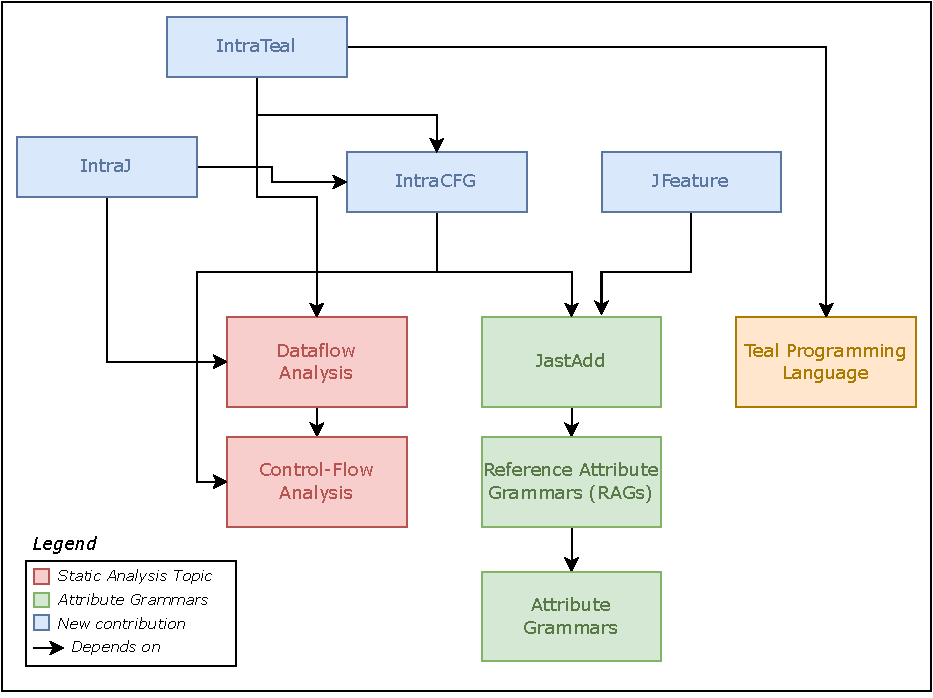
\includegraphics[width=0.9\textwidth]{kappa/img/Dependencies.pdf}
  \caption{\label{fig:dependencygraph}Dependency graph of the concepts discussed in this Section.}
\end{figure}
The dependency graph in Figure~\ref{fig:dependencygraph} shows the relationship between
the concepts and the contribution of this thesis.

\subsection{Automatic Program Analysis: Positioning My Research Within the Field}
Automatic Program Analysis is a branch of computer science that aims to automatically
analyse and evaluate programs' properties, e.g., \emph{correctness}, \emph{liveness} and \emph{safety}. We can distinguish two main
approaches to program analysis: \emph{static} and \emph{dynamic} analysis.

Dynamic analysis examines the behaviour of a program by executing it.
Precise information about a single program's execution are gathered
and used to determine the properties of the program.
This approach is effective in detecting runtime errors, such as memory leaks~\cite{Valgrind},
performance bottlenecks~\cite{VTune}, and security vulnerabilities~\cite{li2018fuzzing}.
However, its limitations come from the requirement for complete and
accurate input data for a single run, and the difficulty in accounting for
all possible execution paths.

In contrast, static analysis performs the analysis without executing the program,
relying on information gathered from the source code. This approach has
the advantage of being more exhaustive, as it can analyse the entire program,
including infeasible execution paths. However, a limitation of static analysis is
that it is prone to producing false positive results, since it cannot take into
account the actual behaviour of the program at runtime.

Static Analysis can be further divided into several categories, including \emph{Type}
and \emph{Effect analyses}~\cite{nielson1999type}. Type Analysis aims to determine the type of variables and expressions
in a program, which can be used to identify type mismatches, type errors, and improve
code readability. Effect analysis focuses on the study of side effects that a program can
produce, such as the mutation of data. This information can be used to identify
potential bugs and improve program understandability.

In the context of this thesis, we focus on intraprocedural control-flow and dataflow analysis, which
involve analysing the flow of data within a single procedure in a program.
This type of analysis is both a type and effect analysis, as it not only considers
the types of data being operated on, but also the effects of operations on the
flow of data within the procedure.
We do this using Monotone Frameworks, a mathematical framework that provides a
foundation for dataflow analysis. In the future, we aim to improve the precision of the analysis
by considering the implementation of interprocedural analysis, which involves
analysing the flow of data across multiple procedures in a program.

Additionally, precision is a crucial aspect of dataflow analysis.
Depending on the desired outcome, various levels of precision can be achieved,
but it is important to weigh the trade-off between precision and performance.
A higher level of precision often requires increased computational resources,
leading to a decrease in performance, and vice versa. Hence, finding the right
balance between precision and performance is crucial in achieving effective and
efficient dataflow analysis results.

In the context of our research, we have chosen to compute control-sensitive and
exception-sensitive control-flow analyses. This approach
simplifies the specification of dataflow analyses which are built upon the
control-flow analysis.

In terms of implementation strategies, there are various approaches that can be
used, including Datalog~\cite{dura2021javadl}, functional programming~\cite{madsen2016datalog}, or ad-hoc implementation.
However, we choose to implement the analysis using Reference Attribute Grammars.
This approach allows us to exploit the benefits of modularity, high-level programming,
and on-demand evaluation, which results in a flexible and efficient implementation.

We recognise that the results of our analyses, while effective,
may not be sound nor complete and that the analysis may not be able to identify
all the bugs or vulnerabilities in a program~\cite{livshits2015defense}.





\subsection{Control-flow analysis}
Control-flow analysis refers to the computation of
 the execution and evaluation order of the program's statements and expressions.
Each possible evaluation order of a program is called a control-flow path.
The result of the control-flow analysis is a control-flow graph (CFG) $G=(V,E)$.
Each vertex $v \in V$ represents a unit of execution, e.g., a single statement or expression,
or a basic block (a sequence of statements without labels and jumps).
Each edge $(v_1,v_2) \in E$  represents a control-flow edge, indicating that the
execution of $v_1$ may be directly followed by the execution of $v_2$.

We can distinguish two main approaches to constructing the CFG for a program:
on the source level and the intermediate representation (IR). The source-level approach
involves analysing the source code of a program and constructing the CFG
directly from the source code on top of the abstract syntax tree. The IR approach involves
first converting the source code into an IR, e.g., bytecode,
and then constructing the CFG from the IR.%

The construction of the CFG at the source level presents several advantages. One of the
main benefits is the ability to map the analysis results directly back to the source code
and present it to the user in the context of the original program. On the other hand,
if the CFG is constructed at the IR level, there would be a complex translation step
required to find the corresponding source level constructs, and in some cases it would
not even be possible due to the loss of information during the translation process, e.g.,
\code{source-file retention} policy for Java annotations.
For this reason, constructing the CFG at the source level is particularly useful for
debugging and program understanding tasks, as it provides a clear and direct
representation of the program. Additionally, this approach enables faster and
more efficient analysis as it eliminates the overhead of IR generation and can
also handle semantically and syntactically invalid code, making it useful for
analysing programs with errors or incomplete code. Furthermore, in situations where
IR generation must occur in real-time, such as when the analysis is performed in an
IDE, the overhead of code generation and optimisation may cause latency in the IDE and frustration for the developer~\cite{piskachev2022far}.
In these cases, constructing the CFG at the source level may be a more efficient option.

However, there are also some disadvantages to constructing the CFG on the source level.
One of the main limitations is that it can be more difficult to accurately capture the
control-flow of a program since the source code may contain unsugared constructs,
such as macros and preprocessor directives, that
can complicate the analysis specification. In addition, the source code may be written in a variety
of languages with different syntax and semantics, making it challenging to
design a single analysis that works across all languages.

The examples in Figures~\ref{fig:cfgsourcelevel} and~\ref{fig:cfgintermediatelevel} show the source-level and bytecode control-flow
graphs of the simple method \texttt{foo}. To simplify dataflow analyses, it is
a common practice to add two additional nodes to the CFG, the \emph{Entry}
and \emph{Exit} nodes. These nodes represent the unique entry and exit points of the method, respectively.
\begin{figure}[h]
  \centering
\begin{tabular}{l r}
  \begin{lstlisting}[language=JastAdd]
void foo(){
  Integer x = 0;
  if (x > 0) {
    x = 1;
  } else {
    x = null;
  }
}
  \end{lstlisting} &\hspace{2.5cm}
  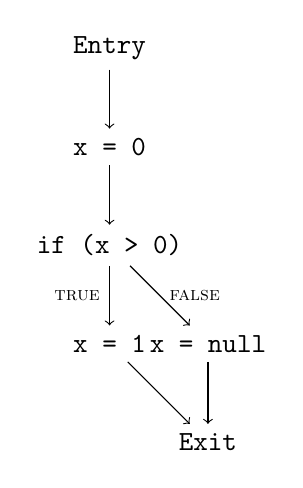
\begin{tikzpicture}[node distance=1.25cm, baseline=(current bounding box.center)]
      \node (start) [rectangle] {\texttt{Entry}};
      \node (assign) [rectangle, below of=start] {\texttt{x = 0}};
      \node (if) [rectangle, below of=assign] {\texttt{if (x > 0)}};
      \node (then) [rectangle, below of=if] {\texttt{x = 1}};
      \node (else) [rectangle, right of=then] {\texttt{x = null}};
      \node (end) [rectangle, below of=else] {\texttt{Exit}};
      \draw [->] (start) -- (assign);
        \draw [->] (assign) -- (if);
      \draw [->] (if) -- node [left, font=\scriptsize] {\textsc{true}} (then);
      \draw [->] (if) -- node [right,  font=\scriptsize]{\textsc{false}} (else);
      \draw [->] (then) -- (end);
      \draw [->] (else) -- (end);
  \end{tikzpicture}
  \end{tabular}
  \caption{\label{fig:cfgsourcelevel}Source level control-flow graph of the \texttt{foo} method, showing the branching behaviour of the if statement.}
\end{figure}


\begin{figure}[h]
  \centering
\begin{tabular}{l r}

\begin{lstlisting}[language=bytecode, frame=none]
1 : 0 : iconst_0
2 : 1 : invokestatic  #7
3 : 4 : astore_1
4 : 5 : aload_1
5 : 6 : invokevirtual #13
6 : 9 : ifle          20
7 : 12: iconst_1
8 : 13: invokestatic  #7
9 : 16: astore_1
10: 17: goto          22
11: 20: aconst_null
12: 21: astore_1
13: 22: return
\end{lstlisting}
&\hspace{2.5cm}
\scalebox{0.85}{
\begin{tikzpicture}[
  node distance=0.25cm,
  every node/.style={shape=rectangle, align=center},
  baseline=(current bounding box.center)]
  % Nodes
  \node (0) {0};
  \node (1) [below=of 0] {1};
  \node (2) [below=of 1] {2};
  \node (3) [below=of 2] {3};
  \node (4) [below=of 3] {4};
  \node (5) [below=of 4] {5};
  \node (6) [below=of 5] {6};
  \node (7) [left=of 6] {7};
  \node (8) [below=of 7] {8};
  \node (9) [below=of 8] {9};
  \node (10) [below=of 9] {10};
  \node (11) [right=of 6] {11};
  \node (12) [below=of 11] {12};
  \node (14) [below=of 6] {};
  \node (15) [below=of 14] {};
  \node (16) [below=of 15] {};
  \node (13) [right=of 10] {13};
  \node (exit) [right=of 13] {\texttt{exit}};
  \node (entry) [left=of 0] {\texttt{entry}};

  % Edges
  \path[-stealth] (0) edge (1);
  \path[-stealth] (1) edge (2);
  \path[-stealth] (2) edge (3);
  \path[-stealth] (3) edge (4);
  \path[-stealth] (4) edge (5);
  \path[-stealth] (5) edge (6);
  \path[-stealth] (6) edge[bend right] (7);
  \path[-stealth] (6) edge[bend left] (11);
  \path[-stealth] (7) edge (8);
  \path[-stealth] (8) edge (9);
  \path[-stealth] (9) edge (10);
  \path[-stealth] (10) edge (13);
  \path[-stealth] (11) edge (12);
  \path[-stealth] (12) edge (13);

  % \path[->] (0) edge (1) (1) edge (2) (2) edge (3) (3) edge[bend right] (6) (3) edge[bend left] (11) (6) edge (7) (7) edge (8) (8) edge (13) (11) edge (12) (12) edge (13);
  \path[-stealth] (13) edge (exit) (entry) edge (0);
   \draw[dashed] (0.north west) rectangle (1.south east);
   \draw[dashed] (2.north west) rectangle (2.south east);
   \draw[dashed] (3.north west) rectangle (5.south east);
   \draw[dashed] (6.north west) rectangle (6.south east);
   \draw[dashed] (7.north west) rectangle (8.south east);
   \draw[dashed] (9.north west) rectangle (10.south east);
   \draw[dashed] (11.north west) rectangle (12.south east);
   \draw[dashed] (13.north west) rectangle (13.south east);
  % \draw[dashed] (6.north west) rectangle (8.south east);
  % \draw[dashed] (11.north west) rectangle (12.south east);

\end{tikzpicture}}
\end{tabular}
\caption{\label{fig:cfgintermediatelevel}Bytecode control-flow graph of the \texttt{foo} method. Each dashed box represents a basic block.}
\end{figure}




\subsection{Dataflow Analysis}
\label{sec:dataflowanalysis}
Dataflow analysis is a technique used in computer science to analyse the flow of
data through a program. It has its roots in the field of program optimisation,
where it was initially used to identify opportunities for improving the performance
of programs by tracking variable definitions and uses. This information can be used to optimise the program by eliminating
unnecessary computations (e.g., Very Busy Expression or Available Expression
analyses~\cite{aho2007compilers}) and improving
the use of available resources (e.g., registers optimisation).


In the context of bug detection, dataflow analysis can be used to identify
potential sources of errors in a program by tracking the flow of data through
the program and identifying points where data may be used in unexpected or
incorrect ways. This can be particularly useful in identifying bugs that may
not be immediately apparent, such as those that only occur under certain
conditions or when certain combinations of input data are used (e.g., \texttt{IndexOutOfBound} exception).
Many static analysis tools for Java programs, e.g., FindBugs, employ intraprocedural
data-flow analysis to identify potential bugs in Java code.
% I looked here how they cited pmd, findbugs and spotbugs. https://ieeexplore.ieee.org/stamp/stamp.jsp?tp=&arnumber=8103456
Dataflow analysis, particularly interprocedural dataflow analysis, is widely
used to identify potential security vulnerabilities in software~\cite{flowdroid}. 
In fact, an interprocedural control-flow graph enables tracking of the flow of 
sensitive across multiple methods or functions, thereby allowing identification of points
where the data may be exposed to unauthorized access or manipulation.

We will demonstrate the application of dataflow analysis by presenting the following
practical example. Let us reconsider the \code{foo} method introduced in Figure~\ref{fig:cfgsourcelevel}.
Our goal is to determine at each stage of the program whether the variable \code{x}
has a \code{null} value or not\footnote{For simplicity, we assume that the language
allows only assignments of the form \code{x = y} where \code{x} and \code{y} can
be either variables a numeric constants or the \code{null} literal.}.
 At the entry point of the method, i.e., Entry node,
it is indeterminate whether \code{x} is \code{null} or not, as it has not been initialized yet.
However, at the declaration of the variable \code{x}, we can determine that it is
not \code{null} because it is initialised to a non-\code{null}
value. Then, if the condition \code{if(x > 0)} is \code{true}, the
variable \code{x} is assigned a new value, which is not \code{null}. If the condition
is \code{false}, the variable \code{x} is assigned to \code{null}. Therefore, at the
end of the method, the variable \code{x} may be either \code{null} or not \code{null}.
This information can be used to identify potential bugs in the program, such as
\code{NullPointerException}.

We keep track of the value of \code{x} by mapping it to a finite set of possible values:
\code{null}, \code{notnull}, \code{maybenull}, or \code{undefined}.
As we traverse the control-flow graph, we propagate this information from node
$n$ to node $n'$ if $(n,n')\in E$, until it reaches the exit node.

The information is updated at each node $n$ according to the following rules:
\begin{itemize}
\item If $n$ is an assignment node, the information is updated according to the
assignment operation. For example, if the assignment is \code{x = null}, then the
it is recorded that \code{x} is updated to \code{null}. If the assignment is \code{x = y}, then
\code{x} is mapped to the value \code{y} maps to.
\item If $n$ is a conditional, an Entry or an Exit node, no update is performed.
\end{itemize}

The dataflow analysis just described is an instance of the mathematical concept of
Monotone Frameworks~\cite{Nielson2010Principles}.

\subsubsection*{Monotone Frameworks}
\label{sec:monotoneframeworks}
Monotone frameworks are a theoretical approach for reasoning
about program dataflow properties.
This approach provides a flexible and generic framework for expressing and solving
dataflow equations, which can be used to reason about a wide range of dataflow
properties, such as live variables, reaching definitions and available expressions analyses.
Monotone frameworks are built on the concept of lattice~\cite{Donnellan1968}.
A lattice is a partially ordered set in which any two elements have a unique least
upper bound (also known as a join or a supremum) and a unique greatest lower bound
(also known as a meet or an infimum). This means that, for any elements $a$ and $b$ in
the lattice, there exists a unique element denoted as  $a \vee b$  (or  $a \cup b$)
such that  $a \leq a \vee b$  and  $ b \leq a \vee b$, and  $a \wedge b$
(or  $ a\cap b$) such that  $ a\wedge b\leq a$  and  $a \wedge b\leq b$.
A well-formed lattice has a unique least element, commonly denoted as $\bot$,
and a unique greatest element commonly denoted as $\top$. These elements satisfy
the properties that for any element $x$ in the lattice, $\bot \leq x$ and $x \leq \top$.
In dataflow analysis, lattices are widely used to represent the information flow in a program.
A common example of a lattice used in dataflow analysis is the \emph{binary lattice} with
elements \emph{true} and \emph{false}, which is used to represent the presence or absence of
of a property. Another example is the \emph{interval lattice}, which is used
to represent ranges of number. This lattice, compared to the binary lattice, is more
complex but provides more precise information about the flow of numerical values
in a program. Additionally, while the binary lattice is \emph{finite}, the interval lattice can
be potentially \emph{infinite}.
\begin{wrapfigure}{r}{0.5\textwidth}
     \begin{center}
  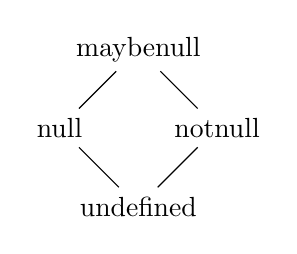
\begin{tikzpicture}
      \node (top) at (0,1) {\code{maybenull}};
      \node (null) at (-1,0) {\code{null}};
      \node (notnull) at (1,0) {\code{notnull}};
      \node (bot) at (0,-1) {\code{undefined}};
      \draw (bot) -- (null) -- (top) -- (notnull) -- (bot);
    \end{tikzpicture}
    \caption{\label{fig:lattice}Diagram of the lattice used in the example in Section~\ref{sec:dataflowanalysis}.
    In this case, \code{maybenull} $= \top$ and \code{undefined}$= \bot$.}
  \end{center}
\end{wrapfigure}


Monotone frameworks include a join operator $\bigsqcup$\footnote{
  For analyses over sets, the join operator can be $\bigcup$ or $\bigcap$.
}, a monotone transfer function $f$,
and a finite lattice $\mathcal{L}$.

In our example, the lattice $\mathcal{L}$ is the set of possible values of the variable \code{x}.
This lattice is shown in Figure~\ref{fig:lattice}. Here \code{maybenull} is
the greatest element in the lattice, as it represents the set of all possible values
that a variable can take. On the other hand, \code{undefined} is the least element
representing the absence of information.
The join operator $\bigsqcup$ merges the information of two nodes by taking their
union. For instance, if node $n$ has information \code{null} and node $n'$ has
information \code{notnull}, then the information at the merged node $n \bigsqcup n'$
becomes \code{maybenull}.
In the previous section, we explained how a node affects the flow of data
using plain language. Now, we will present this concept in a formal manner
as a transfer function. Let \textit{Var} be the set of variables in the program, we define
the monotone transfer function $f_{\textit{NULL}}: (\textit{Var} \rightarrow \mathcal{L}) \times V \rightarrow (\textit{Var} \rightarrow \mathcal{L})$
as follows:

\[
  f_{\textit{NULL}}(\Gamma, \vterminal{node}) =
  \begin{cases*}
  \Gamma[\vmetavar{v} \mapsto \semNPA{\vmetavar{e}}^\Gamma] & if  \vterminal{node} is \vterminal{\vmetavar{v} = \vmetavar{e}}  \\
  \Gamma  & otherwise
\end{cases*} \]%

\[
\begin{array}{llcl}
\textrm{where}&\semNPA{\vterminal{n}\in \mathbb{N}}^\Gamma			&=& \textbf{notnull}\\
&\semNPA{\vterminal{null}}^\Gamma			&=& \textbf{null}\\
&\semNPA{\vmetavar{v}}^\Gamma				&=& \Gamma(\vmetavar{v})\\
\end{array}
\]


To propagate information from node $n$ to its succeeding nodes and to represent the
effect of traversing a node, we define the following two equations:
\begin{align*}
  \text{in}(n) &= \begin{cases} \{ v \rightarrow \bot \mid \forall v \in $\textit{Var}$ \} & $if $ n $ is Entry$ \\ \bigsqcup\limits_{p \in \text{pred}(n)} \text{out}(p) & $otherwise$ \end{cases} \\
  \text{out}(n) &= f_{\mathit{NULL}}(\text{in}(n),n)
\end{align*}
where $\text{pred}(n) = \{ p \mid (p,n)\in E\}$.
We have defined the $in$ and the $out$ sets to model the information that is available
before and after passing through a node, respectively. The $in$ set gathers the available
information before entering the node, while the $out$ set captures the effect
of applying the transfer function $f_{\textit{NULL}}$ on the $in$ set.

These equations can be adapted to perform backward analyses, i.e., analyses that
propagate information from the exit node to the entry node.
Given a monotonic transfer function $f$ and a finite lattice $\mathcal{L}$, the equations for
a backward analysis are defined as follow:
\begin{align*}
  \text{out}(n) &= \bigsqcup\limits_{s \in \text{succ}(n)} \text{in}(s) \\
  \text{in}(n) &= f_n(\text{out}(n),n)
\end{align*}

The equations for both forward and backward analyses define a mutual dependency
between the $in$ and $out$ sets of a node.
This circular dependency is solved through a fix point computation,
a mathematical technique that finds a stable state, or fix point, in a system.
In the context of the Monotone frameworks, this
refers to finding a state where the $in$ and $out$ sets of all nodes in the CFG have reached a
stable value, and no further changes will occur. The fix point is guaranteed to exist
because the transfer function $f$ is monotone~\cite{Knaster1929}.



\subsection{Attribute Grammars}
\label{chap:attr-grammars}
Attribute grammars~\cite{knuth1968semantics} (AGs) are a formalism for specifying
the syntax and semantics of programming languages.
They were first introduced by Knuth in 1968 as a way to define the syntax and semantics of the programming
language ALGOL 68. This formalism is based on the concept of attributes,
which are properties associated with the elements of a language's abstract syntax tree.
Attribute grammars provide a powerful tool for specifying the behaviour of a programming
language and for verifying the correctness of programs written in that language.
%
AGs are composed of two components: a context-free grammar~\cite{CREMERS197586},
which defines the language's syntax, and an attribute evaluation function,
which defines the semantics of the language. Context-free grammar is used to
parse a program into its abstract syntax tree, and the attribute evaluation function
is used to compute the values of the attributes associated with each tree element.

Attribute grammars enable the description of the
interdependence of syntactic and semantic elements of a programming language.
For instance, the type of a variable may be determined by its declaration,
but the type of an expression may be determined by the types of its sub-expressions.
Attribute grammars provide a way to specify these constraints.

Attributes are define using equations. We can distinguish two types of
attributes: synthesized attributes and inherited attributes.
For the sake of readability, we borrow the notation introduced by Fors et al. in~\cite{fors2020patterns},
where attribute names are preceded by a symbol that indicates the type of the attribute.
We reserve the symbol \Abase{x} to denote the attribute name and the symbol $e$ to denote the attribute value,
e.g., a constant, a function of the node's children, or a function of the node's children
and the node's own attributes.

A \emph{synthesized} attribute is a property of a non-terminal that is computed
based on the attributes of its possible derivations. For example, the type of an expression
in a programming language may be a synthesized attribute computed based
on the types of sub-expressions in the expression. For instance, if a variable is initialized
with the expression ``3 + 4'', the variable type would be determined to
be integer based on the types of the operands in the expression.
We denote a synthesized attribute as follows:
\begin{equation*}
  \Asyn{A}{x} = e
  \end{equation*}
where \astnode{A} is the name of the node type.

An \emph{inherited} attribute is a property of a non-terminal that is inherited from
its parent element in the abstract syntax tree.
An example of an inherited attribute is the scope of a variable in a programming
language. The scope of a variable is the region of a program in which the variable
is visible and can be accessed. The scope of a variable is inherited from the
context in which it is declared. For example, if a variable is declared within a
function, the variable will be visible and accessible within the body of the function
but not outside of the function.


Inherited attributes are defined in two parts: a declaration and an equation.
\begin{equation*}
\Ainh{A}{x} \quad\quad \quad\quad \Ainhdef{B}{*}{x} = e
\end{equation*}
where \astnode{A} and \astnode{B} are node types.
The first part of the equation declares the attribute \Ainh{A}{x} as inherited by \astnode{A},
so every node of type \astnode{A}  can access it. The second part of the
equation defines the attribute for each child of \astnode{B}. The wildcard \astnode{*}
indicates that the attribute is defined and broadcasted to all children of \astnode{B} with type \astnode{A}.

\begin{figure}
    \begin{tikzpicture}[scale=0.7,edge from parent/.style={draw,-latex},sibling distance=8em,
      every node/.style = {align=center,scale=1},
      astnode/.style={shape=rectangle, draw, fill=white, minimum width=5mm,%
      minimum height=10mm},
      synthesized/.style={shape=rectangle, draw, fill=orange!15},
      inherited/.style={shape=rectangle, draw, fill=blue!15}
      ]

    \node [astnode,draw] (A) {\code{A}}
      child {node [astnode] (B) {\code{B}}}
      child {node [astnode] (C) {\code{C}}
    }
    ;
    \node [synthesized , draw, right=0pt of A] (AA) {\Asyn{A}{z} = \Asyn{B}{x} + 1 = 3};
    \node [synthesized , draw, left=0pt of B] (BB) {\Asyn{B}{x} = 2};
    \node [synthesized , draw, right=0pt of C] (CC) {\Asyn{C}{v} = 5};
    \node [inherited , draw, below right =0pt of C] (CC) {\Ainh{C}{y} = \Asyn{A}{z} + \Asyn{C}{v} = 8};

    \matrix [draw, below right = -50pt and -180pt,inner sep=1ex,cells={nodes={font=\sffamily,anchor=west}}] at (B) {
      \node [synthesized] {}; & \node{Synthesized attributes}; \\
      \node [inherited] {}; & \node{Inherited attributes}; \\
      \node [rectangle,draw] {}; & \node{AST Node}; \\
      \draw[-latex,dotted,color=black](0,0) -- ++ (0.3,0); & \node{Child relation}; \\
    };
    \end{tikzpicture}
    \caption{\label{fig:ragsExample} Graphical representation of the attribute grammar example.}
\end{figure}

To better explain the concept of AGs, we present the following
example with the following abstract grammar:
    \begin{align*}
        A& ::= B \quad C \\
        B& \\
        C&
    \end{align*}
and the following attribute declarations:
    \begin{align*}
        \Asyn{A}{z}& = \Asyn{B}{x} + 1 \\
        \Asyn{B}{x}& = 2 \\
        \Asyn{C}{v}& = 5 \\
        \Ainh{C}{y}& \\
        \Ainhdef{A}{C}{y}& = \Asyn{A}{z} + \Asyn{C}{v} \\
    \end{align*}
The value for the synthesized attribute \Asyn{A}{z} is computed by solving
the equation systems for the attributes \Asyn{A}{z} and \Asyn{B}{x}:
\begin{align*}
    \Asyn{A}{z} &= \Asyn{B}{x} + 1 \\
    \Asyn{B}{x} &= 2
\end{align*}
leading to \Asyn{A}{z} = 3 and \Asyn{B}{x} = 2.
The value for the inherited attribute \Ainh{C}{y} is defined by node \astnode{A} for
each child of type \astnode{C}. The value of \Ainh{C}{y} is computed by solving the equation system:
\begin{align*}
    \Ainh{C}{y} &= \Asyn{A}{z} + \Asyn{C}{v} \\
    \Asyn{C}{v} &= 5\\
    \Asyn{A}{z} &= 3
\end{align*}
resulting in \Ainh{C}{y} = 8. Figure~\ref{fig:ragsExample} depicts the described example.


\subsection{Reference Attribute Grammars}
\label{sec:rag}
Reference Attribute Grammars (RAGs) were introduced in~\cite{DBLP:journals/informaticaSI/Hedin00}
and are an extension of AGs to Object-Oriented languages. While attributes in AGs
can only refer to terminal values, RAGs allow attributes to refer to non-terminals, i.e., nodes in the AST.
RAGs are well-suited for the analysis of object-oriented languages since they enable
the definition of relations between AST nodes. Attributes referring
to AST nodes can declaratively construct relations, i.e., graphs, on the AST.
Examples of the relations that can be constructed using RAGs are:
\begin{itemize}
    \item Name analysis: checks that all names are well-defined and used correctly. A relation between
    the name and the definition of the name is constructed,
    \item Type analysis: checks that all expressions have a valid type. A relation between the expression
    and its type is constructed,
    \item Graph of a class hierarchy: a graph where nodes are classes and edges are inheritance relations,
    \item Control flow graph: a graph where nodes are statements or expressions, and edges are control flow relations, and,
    \item Call graph: a graph where nodes are methods and edges are method calls.
\end{itemize}

\subsection{The TEAL Programming Language}
\label{sec:teal}
TEAL v0.4 (Typed Easily Analysable Language) is a programming language designed by Christoph Reichenbach and used in the
program analysis\footnote{\url{https://fileadmin.cs.lth.se/cs/Education/EDAP15/2022/web/index.html}} course at Lund University.
TEAL aims to provide a language that allows students to
focus on the challenges of performing program analysis on a real-world language
without being overwhelmed by the details of a fully-featured language.
The concrete and abstract syntax of TEAL-0 are shown in Figure~\ref{fig:tealGrammar}.
One of the key features of TEAL is that it is an object-oriented language,
which means that it allows the creation of classes and objects that can inherit
characteristics and behaviour from one another. However, it does not have a dynamic
dispatcher, which means that the method that is called for an object at run-time
is determined at compile-time based on the type of the object.
TEAL is divided in layers, with each version building
upon the features of the previous one. TEAL-0 is the most basic version and includes
support for variable declarations and use, procedures, and basic control structures such as if
and while statements. TEAL-1 introduces the enhanced-for loop, and TEAL-2 allows users to
define their types.
For simplicity, we will use TEAL-0 and TEAL-1 to exemplify the use of RAGs
and the main results summarized in this thesis.
\newsavebox{\mylistingbox}

\begin{figure}[H]
    \hspace*{-1cm}
    \begin{minipage}{0.5\textwidth}
        \[\footnotesize
        \begin{array}[t]{lcl@{\hspace{0.4cm}}}
          \nta{Program} & \Prod & \ntstar{Decl} \\
          \\
          \nta{Decl} & \Prod & \nt{VarDecl}\ \\
                       & \VB & \vterminal{fun}\ \terminal{id}\ \vterminal{(}\ \ntq{formals}\ \vterminal{)}\\
                       &&  \nt{optTyped}\ \vterminal{=}\ \nt{stmt} \\
          \\
          \nta{VarDecl} & \Prod & \vterminal{var}\ \terminal{id}\ \nt{optTyped} \\
                        & \VB   & \vterminal{var}\ \terminal{id}\ \nt{optTyped}\ \vterminal{:=}\ \nt{Expr} \vterminal{;}\\
          \\
          \nta{formals} & \Prod & \terminal{id}\ \nt{optTyped} \\
                        & \VB & \terminal{id}\ \nt{optTyped}\ \vterminal{,}\ \nt{formals}\\
                      \\
          \nta{optTyped} & \Prod & \vterminal{:}\ \nt{Type}\\
                        & \VB{} & \varepsilon \\
          \\
          \nta{Type} & \Prod & \Cty{int}\ \VB\ \Cty{string}\ \VB\ \Cty{any} \\
                     & \VB   & \Cty{array}\ \Cty{[}\ \nt{Type}\ \Cty{]} \\
          \\
          \nta{Block} & \Prod & \vterminal{\{}\ \ntstar{Stmt}\ \vterminal{\}} \\
          \\
          \nta{Expr} & \Prod & \nt{Expr}\ \nt{binop}\ \nt{Expr} \\
                     & \VB   & \vterminal{not}\ \nt{Expr} \\
                     & \VB   & \vterminal{(}\ \nt{Expr}\ \nt{optTyped}\ \vterminal{)} \\
                     & \VB   & \nt{Expr}\ \vterminal{[}\ \nt{Expr}\ \vterminal{]} \\
                     & \VB   & \terminal{id}\ \vterminal{(}\ \ntq{actuals}\ \vterminal{)} \\
                     & \VB   & \vterminal{[}\ \ntq{actuals}\ \vterminal{]} \\
                     & \VB   & \vterminal{new}\ \nt{Type}\ \vterminal{(}\ \nt{Expr}\ \vterminal{)} \\
                     & \VB   & \terminal{int}\ \VB\ \terminal{string}\ \VB\ \vterminal{null} \\
                     & \VB   & \terminal{id} \\
          \\
          \nta{actuals} & \Prod & \nt{Expr} \\
                        & \VB   & \nt{Expr} \vterminal{,}\ \nt{actuals} \\
          \\
          \nta{binop} & \Prod &
              \vterminal{+}
                      \ \VB\ \vterminal{-}
                      \ \VB\ \vterminal{*}
                      \ \VB\ \vterminal{/}
                      \ \VB\ \vterminal{\%}\\
                      & \VB& \vterminal{==}
                      \ \VB\ \vterminal{!=}\\
                      & \VB&  \vterminal{$<$}
                      \ \VB\ \vterminal{$<=$}
                      \ \VB\ \vterminal{$>=$}
                      \ \VB\ \vterminal{$>$}
                      \\
                      & \VB& \vterminal{or}
                      \ \VB\ \vterminal{and}\\
          \\
          \nta{Stmt} & \Prod & \nt{VarDecl} \\
                     & \VB   & \nt{Expr}\ \vterminal{;} \\
                     & \VB   & \nt{Expr}\ \vterminal{:=}\ \nt{Expr}\ \vterminal{;}\\
                     & \VB   & \nt{Block} \\
                     & \VB   & \vterminal{if}\ \nt{expr}\ \nt{block}\ \vterminal{else}\ \nt{block} \\
                     & \VB   & \vterminal{if}\ \nt{expr}\ \nt{block} \\
                     & \VB   & \vterminal{while}\ \nt{expr}\ \nt{block} \\
                     & \VB   & \vterminal{return}\ \nt{expr}\ \vterminal{;}\\
        \end{array}
      \]
        \end{minipage}%
        \begin{minipage}{0.8\textwidth}
            \hfill
\begin{lrbox}{\mylistingbox}
        \begin{lstlisting}[language=ASTGrammar]
    Program ::= Decl*;

    abstract Decl;
    VarDecl : Decl ::= IdDecl [DeclaredType:Type] [Initializer:Expr];
    FunDecl : Decl ::= IdDecl [DeclaredReturnType:Type] Formal:VarDecl* [Body:Stmt];

    abstract Expr;
    abstract BinExpr : Expr ::= Left:Expr Right:Expr;
    AddExpr : BinExpr;
    SubExpr : BinExpr;
    MulExpr : BinExpr;
    DivExpr : BinExpr;
    ModExpr : BinExpr;
    EQExpr  : BinExpr;
    NEQExpr : BinExpr;
    LTExpr  : BinExpr;
    GTExpr  : BinExpr;
    LEQExpr : BinExpr;
    GEQExpr : BinExpr;
    OrExpr  : BinExpr;
    AndExpr : BinExpr;
    CallExpr : Expr ::= IdUse Actual:Expr*;
    Null : Expr;
    ArrayLiteralExpr : Expr ::= Expr*;
    IndexExpr : Expr ::= Base:Expr Index:Expr;
    NotExpr : Expr ::= Expr;
    TypedExpr : Expr ::= Expr DeclType:Type;
    NewExpr : Expr ::= Type Actual:Expr*;
    Access : Expr ::= IdUse ;

    abstract Constant : Expr;
    IntConstant : Constant ::= <Value:Long>;
    StringConstant : Constant ::= <Value:String>;

    abstract Stmt;
    VarDeclStmt : Stmt ::= VarDecl;
    ExprStmt : Stmt ::= Expr;
    AssignStmt : Stmt ::= LValue:Expr RValue:Expr;
    Block : Stmt ::= Stmt*;
    IfStmt : Stmt ::= Cond:Expr Then:Stmt Else:Stmt;
    WhileStmt : Stmt ::= Cond:Expr Body:Stmt;
    ReturnStmt : Stmt ::= Expr;
    SkipStmt : Stmt;

    IdUse ::= <Identifier>;
    IdDecl ::= <Identifier>;
        \end{lstlisting}
\end{lrbox}
\scalebox{0.75}{\usebox{\mylistingbox}}

        \end{minipage}
\caption{\label{fig:tealGrammar} The concrete and part of the abstract grammar of the \textsc{Teal} language.}
\end{figure}


\subsection{The \textsc{JastAdd} Metacompiler}
\label{sec:jastadd}
The \textsc{JastAdd} metacompiler~\cite{DBLP:journals/entcs/HedinM01} is a powerful tool for constructing
RAGs.
\textsc{JastAdd} allows language designers to handle complex language constructs in a modular and extensible
manner through the use of the RAGs formalism.
The \textsc{JastAdd} metacompiler is a Java-based tool that generates
Java code from a RAG specification. The generated code can be used to construct an AST and to perform
analysis on the AST.
Another important aspect of \textsc{JastAdd} is its support for on-demand attribute evaluation.
Attribute evaluation is performed only when the corresponding
attribute is required and triggered by the program. This approach enables \textsc{JastAdd} to
avoid performing unnecessary computations, which can improve the run-time
performance of the generated program.

The \textsc{JastAdd} metacompiler is based on the following components:
\begin{itemize}
    \item The \textsc{JastAdd} language: a language for the definition of RAGs.
    The \textsc{JastAdd} language is used to specify the abstract grammar of a language and,
    with a Java-like syntax, the attributes of the RAG.
    \item The \textsc{JastAdd} compiler: that is a compiler that generates Java code from a RAG.
\end{itemize}
In \textsc{JastAdd}, synthesized attributes are defined using the \code{syn} keyword followed
by the type and the name of the attribute. Similarly, inherited attributes are defined
using the \code{inh} keyword.

Let us reconsider the example depicted in Figure~\ref{fig:ragsExample}.
The abstract grammar is defined in a ``\code{.ast}'' file with the following syntax:
    \begin{lstlisting}[language=JastAdd]
        A ::= B C;
        B;
        C;
    \end{lstlisting}
where each line defines a non-terminal, i.e., a node in the AST.
The attributes are defined in a ``\code{.jrag}'' file with the following syntax:
    \begin{lstlisting}[language=JastAdd]
        syn int A.z() = B.x() + 1;
        syn int B.x() = 2;
        syn int C.v() = 5;
        inh int C.y();
        eq A.C.y() = A.z() + C.v();
    \end{lstlisting}
The last line is the equation that defines the value of the inherited attribute \Ainh{C}{y} for each child of \astnode{A} of type \astnode{C}.
\begin{figure}
    \begin{center}
        \begin{tikzpicture}
            \tikzstyle{block} = [rectangle, draw, text centered, minimum height=8em, minimum width=8em]
            \tikzstyle{line} = [draw, -latex]
            \node [block] (A) {
                \begin{lstlisting}[language=JastAdd]
aspect AttrDecl {
  syn int A.x() = 1;
  syn int B.x() = 2;
}
                \end{lstlisting}
            };
            \node [block, right=of A, yshift=5em] (B) {
                \begin{lstlisting}[language=JastAdd]
class A {
    public int x(){
        return 1;
    }
}
                \end{lstlisting}
            };
            \node [block, below=of B] (C) {
                \begin{lstlisting}[language=JastAdd]
class B {
    public int x(){
        return 2;
    }
}
                  \end{lstlisting}
             };

             \node (v1) at (-1.5,-0.05) {};
             \node (v2) at (1.7,-0.05) {};
             \node (v3) at (3,1.1) {};
             \node (v4) at (6.3,1.1) {};
             \node (v5) at (6.3,2.3) {};
             \node (v6) at (3,2.3) {};
             \node (v7) at (1.7,0.3) {};
             \node (v8) at (-1.5,0.3) {};
             \draw[opacity=0.2,fill=blue] (v1.center)--(v2.center)--(v3.center)--(v4.center)--(v5.center)--(v6.center)--(v7.center)--(v8.center)--(v1.center);

             \fill [opacity=0.2,blue]
                 (v1) \foreach \i in {2,...,8}{ -- (v\i) } -- cycle;

            \node (vv1) at (-1.5,-0.1) {};
            \node (vv2) at (1.7,-0.1) {};
            \node (vv3) at (3,-1.5) {};
            \node (vv4) at (6.3,-1.5) {};
            \node (vv5) at (6.3,-2.8) {};
            \node (vv6) at (3,-2.8) {};
            \node (vv7) at (1.7,-0.45) {};
            \node (vv8) at (-1.5,-0.45) {};
            \draw[opacity=0.2,fill=red] (vv1.center)--(vv2.center)--(vv3.center)--(vv4.center)--(vv5.center)--(vv6.center)--(vv7.center)--(vv8.center)--(vv1.center);

            \fill [opacity=0.2,red]
                (v1) \foreach \i in {2,...,8}{ -- (vv\i) } -- cycle;
        \end{tikzpicture}
    \end{center}
    \caption{\label{fig:interType} Example of intertype declaration.}
\end{figure}


Another key feature of \textsc{JastAdd}  is the support of \emph{intertype declarations} for the definition of attributes.
An intertype declaration of an attribute is a declaration that is performed into
an aspect\footnote{See \emph{Aspect-Oriented Programming}~\cite{Kiczales1997Aspect}.} that, at compile-time,
is inlined in the class specified in the intertype declaration. The example in Figure~\ref{fig:interType}
shows an intertype declaration of an attribute.
The attributes \Asyn{A}{x} and \Asyn{B}{x} are defined in the aspect \code{AttrDecl}
that is inlined in the classes \code{A} and \code{B}, respectively.

\textsc{JastAdd} supports not only synthesized and inherited attributes, but also:
\begin{itemize}
    \item \emph{Parametrised Attribute}: the value of the attribute might depend
    not only on the AST node itself, but also on the value of the arguments supplied
    to it. Attributes of this kind are widely used, especially in the definition of
    type-checking rules.
    \begin{lstlisting}[language=JastAdd]
syn boolean Type.compatibleType(Type t){
    return this==t;
}
    \end{lstlisting}

    \item \emph{Higher-Order Attribute (HOA)}\footnote{Also known as \emph{Non-Terminal Attributes (NTA)}.}:
    the value of an HOA is a freshly new subtree. They are called \emph{Higher-Order Attributes}
    because they are attributes and, at the same time, non-terminal; therefore, they can be attributed.
    The subtree computed by an HOA behaves like a normal non-terminal, i.e., it can be
    attributed and used in the definition of other attributes. In \textsc{JastAdd}, HOAs
    are defined using the \code{nta} keyword. HOAs are widely used to reify information
    that is not explicit in the source code and, therefore, not present in the AST.
    For example, we use HOAs to reify a method's entry and exit points. In CFGs, it
    is common to have a unique entry point and exit point for each method.
    \begin{lstlisting}[language=JastAdd]
syn nta Entry FunDecl.entry() = new Entry();
syn nta Exit FunDecl.exit() = new Exit();
    \end{lstlisting}
    We use the right-arrow symbol to denote HOAs, e.g.,  \Ahoa{FunDecl}{entry} and \Ahoa{FunDecl}{exit}.
    \item \emph{Circular Attribute}: an attribute which definition might depend directly
    or indirectly on itself. In \textsc{JastAdd}, circular attributes are expressed using the \code{circular}
    keyword. To guarantee termination, circular attributes are evaluated in a fixed-point
    computation, i.e., the attribute is evaluated until the value of the attribute does not change.
    The requirements, that are not checked by \textsc{JastAdd}, to guarantee termination are:
    \begin{itemize}
        \item All the possible values computed by the attribute must be placed
        in a lattice of finite height.
        \item The intermediate results of the fix-point algorithm must increase
        or decrease monotonically\footnote{In this Thesis, boolean circular attributes start
        as \emph{false} and monotonically grow with $\vee$, while set-typed circular attributes
        start as the empty set and monotonically grow with $\cup$.}.
    \end{itemize}
    We use the symbol \AcircSyn{A}{x} to denote a circular synthesized attribute.

    \item \emph{Collection Attribute}: these attributes have no equations but contributions. The
    result of a collection attribute is the aggregation of contributions that can
    come from anywhere in the AST. A contribution clause is associated with
    an AST node type and describes the information to be included in a collection
    attribute, possibly under certain conditions. Collection attributes are especially
    useful in compiler construction to collect all the semantic errors in a program
    from anywhere in the AST. In \textsc{JastAdd}, collection attributes are defined using the
    \code{coll} keyword.

    An example of a collection attribute is the following:
    \begin{lstlisting}[language=JastAdd]
coll Set<Errors> Program.errors();
Expr contributes this when type.compatible(expectedType()) to Program.errors();
    \end{lstlisting}
    The collection attribute, \texttt{Program.errors()}, denoted with \Acoll{Program}{errors},
    is used to collect all the semantic errors in the program. The contribution clause
    states that the expression \texttt{this} contributes to the collection when
    the expression type is incompatible with the expected type.
\end{itemize}




